\section{Framework}
\label{sec:method}

\begin{figure*}[t]
    \centering
    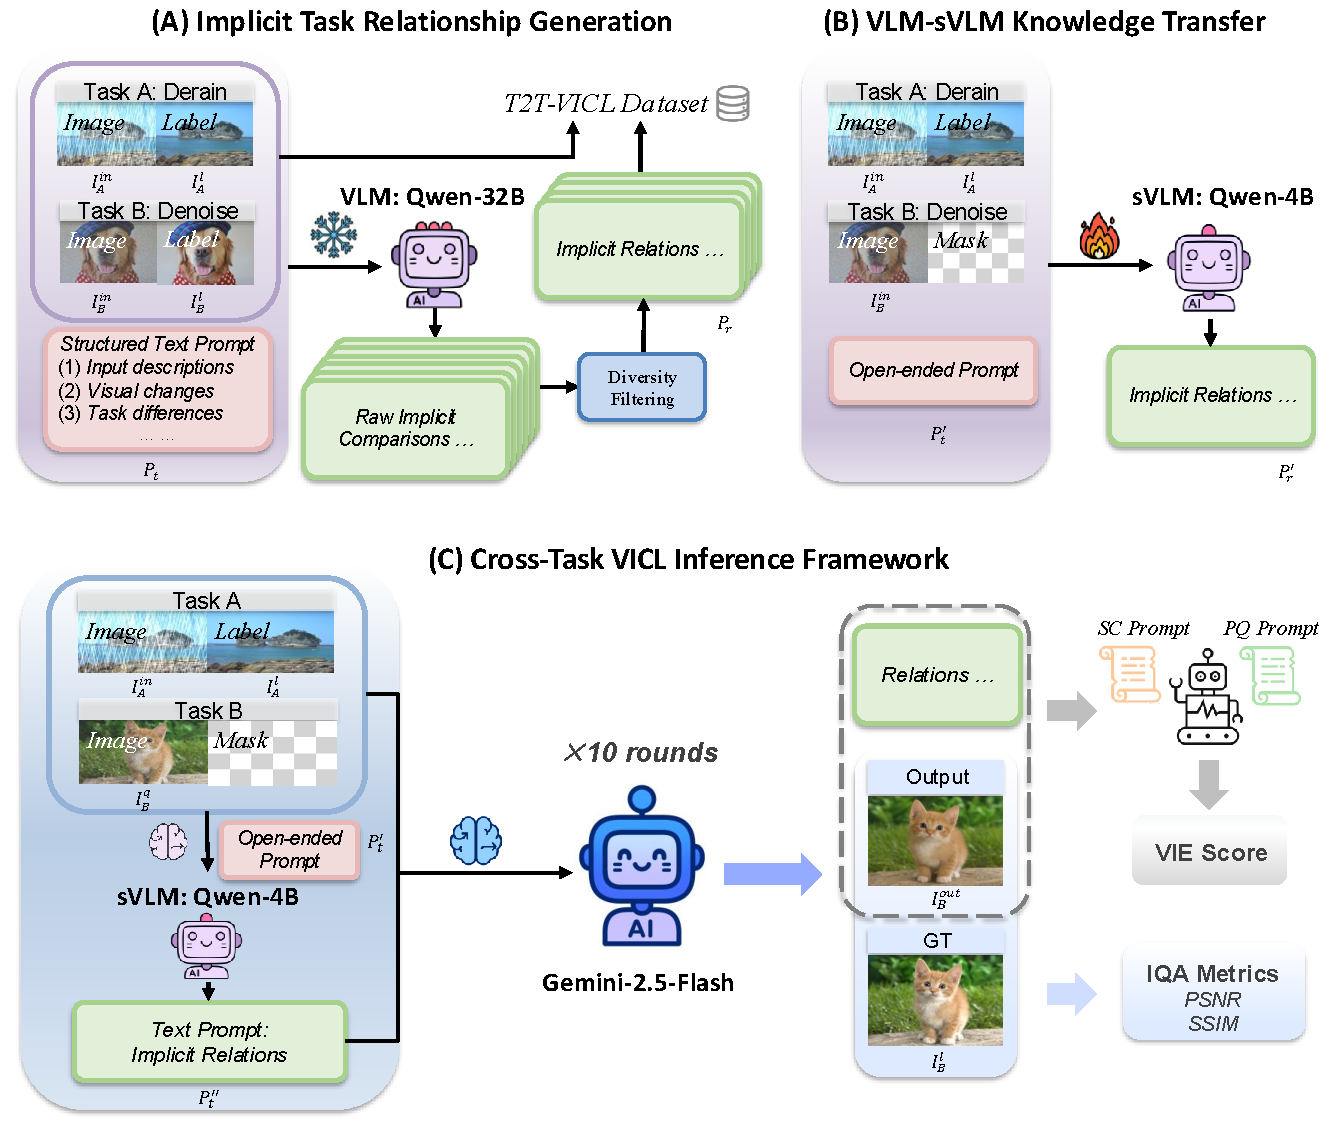
\includegraphics[width=0.88\textwidth]{fig/figure2simple.pdf}
    \caption{Overview of the Proposed Pipeline and its Workflow}
    \label{fig:fig2}
\vspace{-8pt}
\end{figure*}

\subsection{T2T-VICL: Overview of VLM Pipeline}
To explore the boundaries of cross-Task VICL via VLMs, we propose T2T-VICL, a collaborative pipeline that leverages the complementary strengths of large and small language VLMs to enhance vision-language reasoning. First, a large pre-trained VLM generates implicit textual descriptions for two distinct tasks, while the linguistic reliability of these descriptions is quantitatively evaluated. To enable efficient deployment, we fine-tune a sVLM to transfer the reasoning capabilities of the large model while reducing computational overhead. During inference, the sVLM produces text prompts to the final large VLM, thereby guiding the downstream reasoning process. Our main VLM inference pipeline aligns with the standard VICL setting, while the trained sVLM is only an auxiliary component which extracts implicit task descriptions from visual examples and generates text prompts without altering the main inference branch. Finally, candidate results are ranked by another VLM with a visual instruction-guided metric and IQA metrics, and the optimal outcome is selected from the top-k candidates.

\subsection{Implicit Relationship Generation}
We begin by automatically generating rich textual descriptions that implicitly capture the differences between two low-level vision tasks. We consider 12 diverse low-level tasks into three categories as Table~\ref{tab:1}, spanning classic degradation problems (deraining, dehazing, denoising, deblurring, demoireing), removal tasks (shadow removal, reflection removal) as well as generation/enhancement tasks (colorization, low-light enhancement, harmonization, inpainting, style transfer). For any arbitrary pair of tasks A and B, our goal is to obtain an implicit text prompt that depicts the difference without explicitly naming either task. To accomplish this, we leverage large vision-language model Qwen2.5-VL-32B-Instruct, which takes two image pairs as input. We design the text prompt $P_t$ to provide structured comparisons of two tasks: (1) image descriptions---the basic content of the figures from task A and B; (2) visual changes---observable image-level changes, as opposed to labels for each task; and (3) task differences---the perceptible improvements or modifications after applying the task. Crucially, the prompt instructs the VLM to compare these aspects for task A versus task B without explicitly pushing the model to know the task name (not tell the model what exactly the tasks should do), ensuring the description is extremely implicit. This mechanism forces the VLM to articulate the subtle differences in a narrative manner. Meanwhile, we also consider the baseline setting, where the VLM performs VICL with a fixed prompt. Details of the implicit and fixed prompts are provided in Appendix Sec.~\ref{sec:prompt}.

% \begin{table}[h!]
% \centering
% \caption{Categorization of Low-Level Vision Tasks}
% \begin{tabular}{p{2.5cm} p{5.5cm}}
% \hline
% \textbf{Category} & \textbf{Tasks} \\ \hline
% \textbf{Restoration} & Deblurring, Dehazing, Denoising, Deraining, Demoireing \\[3pt]
% \textbf{Removal} & Reflection Removal, Shadow Removal \\[3pt]
% \textbf{Generation / Enhancement} & Style Transfer, Light Enhancement, Colorization, Harmonization \\ \hline
% \end{tabular}
% \label{tab:task_categories}
% \end{table}

% \begin{table}[h!]
% \centering
% \caption{Categorization of Low-Level Vision Tasks}
% \begin{tabular}{p{2.8cm} p{5.4cm}}
% \hline
% \textbf{Category} & \textbf{Tasks} \\ \hline
% \textbf{Restoration} & Deblurring, Dehazing, Denoising, Deraining, Demoireing \\[3pt]
% \textbf{Removal} & Reflection Removal, Shadow Removal \\[3pt]
% \textbf{Generation / Enhancement} & Style Transfer, Light Enhancement, Colorization, Harmonization \\[3pt]
% \textbf{Cross-Task Combination} & Inter-category compositions such as   Deblurring $\rightarrow$ Demoireing or Intra-category compositions such as Reflection Removal $\rightarrow$ Dehazing \\ \hline
% \end{tabular}
% \label{tab:task_categories}
% \end{table}

\begin{table}[!ht]
\vspace{-6pt}
\centering
\footnotesize
\captionsetup{width=0.99\columnwidth, skip=4pt, type=table}
\caption{Categorization of low-level vision tasks. Based on this, we divide cross-task pairs into \textbf{intra-category} compositions such as ``Deblurring $\rightarrow$ Demoireing'', and \textbf{inter-category} compositions such as ``Reflection Removal $\rightarrow$ Dehazing''.}
\vspace{-1pt}
\renewcommand{\arraystretch}{1}
\begin{tabularx}{\columnwidth}{p{0.24\columnwidth} X}
\hline
\textbf{Category} & \textbf{Tasks} \\ \hline
\rowcolor{lightred!30}
\textbf{Restoration} & \makecell[l]{Deblurring, Dehazing, Demoireing, \\Denoising, Deraining} \\
\rowcolor{lightyellow!30}
\textbf{Removal} & Reflection Removal, Shadow Removal \\
\rowcolor{lightblue!30}
\textbf{Generation\slash Enhancement} & Colorization, Harmonization, Inpainting, Light Enhancement, Style Transfer \\
\hline
\end{tabularx}
\label{tab:1}
\vspace{-6pt}
\end{table}


Subsequently, the above procedure is implemented for all the included low-level tasks to build a high-quality benchmark dataset. For each pair of tasks A and B, we sampled a large number of combinations from public datasets and queried the VLM with each sample to get a text output: (i) an input image $I_A^{in}$ and its label $I_A^{l}$ from task A, and (ii) an input image $I_B^{in}$ with the label $I_B^{l}$ from different task B. Thus we obtained the implicit textural relations:
\begin{equation}
P_r = M_l(I_A^{in}, I_A^{l}, I_B^{in}, I_B^{l}, P_t),
\end{equation}
The model is trained to generate the corresponding comparison text that the teacher (32B model) had produced for that pairing. However, the VLM can sometimes produce repetitive or overly generic statements, especially if many samples share similar traits. We therefore conducted a diversity filtering method by using semantic sentence embeddings. We encoded each candidate description with a SentenceTransformer~\cite{reimers2019sentence} (all-MiniLM-L6-v2) to obtain a dense vector representation. This allowed us to quantitatively measure similarities among the descriptions. We then performed clustering in embedding space to detect groups of near-duplicates or redundant phrasing. In this manner, we filtered out repetitive outputs and retained only one representative with the most distinct descriptions. Ultimately, we kept 2,000 diverse descriptions per task pair. To our knowledge, this is the first text-and-image dataset that implicitly captures cross-task relationships, providing the foundation for our next steps.


%\textcolor{blue}{
%\textbf{Datasets and tasks.} We curate twelve low-level vision tasks with canonical sources widely adopted in prior work \textcolor{red}{Add ref}: deblurring (GOPRO), dehazing (D-HAZY), demoireing (UHDM), denoising (SIDD), deraining (RainCityscapes), harmonization (iHarmony4), inpainting (modified DIV2K), colorization (modified DIV2K), low-light enhancement (LoL), reflection removal (SIR$^2$), shadow removal (ISTD), and style transfer (Night2Day). This mix spans degradations (blur, haze, noise, weather streaks, reflections, shadows) and generative transformations (recoloring, illumination/style changes), giving broad coverage for cross-task comparisons used in our framework.}

%\textcolor{blue}{
%\textbf{VLM-as-analyst protocol.} We employ Qwen2.5-VL-32B-Instruct as a descriptive oracle that receives two task exemplars—typically an input→output pair from task A and an input→output pair from task B—together with a structured comparative prompt. The model is instructed to articulate, for each task: (i) the target goal (what the transformation achieves), (ii) the input degradation (artifact type), and (iii) the perceptual changes from input to output. This forces the VLM to reason about abstract phenomena (e.g., global haze veil vs. localized rain streaks, loss of sharpness vs. sensor noise) rather than only recognizing objects. In a practical variant used during data conversion, we sometimes reveal only B's input (no B output) and explicitly ask the model to infer B's transformation type—encouraging robustness to partially observed task pairs.}

%\textcolor{blue}{
%\textbf{Scaling and filtering.} For every ordered task pair, we sample many image examples and query the oracle repeatedly to obtain 2000+ comparative narratives. Because raw generations may be redundant, we embed each description using SentenceTransformer (all-MiniLM-L6-v2), cluster in embedding space, and retain diverse, informative representatives (unused images are reserved for final inference). The result is a curated text corpus that externalizes inter-task relations in natural language.}

%\textcolor{blue}{
%\textbf{Positioning to prior art.} Earlier approaches quantify task affinity with embeddings or transfer matrices (e.g., Task2Vec: Task Embedding for Meta-Learning [https://arxiv.org/abs/1902.03545]; Taskonomy: Disentangling Task Transfer Learning [https://arxiv.org/abs/1804.08328]), which are effective but opaque. Concurrently, language has been used to control restoration models via prompts or instructions (PromptIR: Prompting for All-in-One Blind Image Restoration [https://openreview.net/forum?id=KAlSIL4tXU]; InstructIR: High-Quality Image Restoration Following Human Instructions [https://arxiv.org/abs/2401.16468]; Perceive-IR: Learning to Perceive Degradation Better for All-in-One Image Restoration [https://arxiv.org/abs/2408.15994]). Our contribution is complementary: we use a large VLM to produce textual explanations that act as human-interpretable supervision for cross-task reasoning, rather than as mere control signals. These narratives constitute a language-guided, interpretable proxy for task affinity that we subsequently transfer to a compact model.}


%Traditional task transfer frameworks often quantify inter-task similarity through performance gains or learned embeddings – for example, Taskonomy's transfer matrix or vectorial task embeddings like Task2Vec (Task2Vec: Task Embedding for Meta-Learning [https://arxiv.org/abs/1902.03545]). While such metrics yield a coarse quantitative affinity between tasks, they offer little in terms of human intuition or why certain tasks relate. In this work, we pivot to a qualitatively rich, language-centric approach: we leverage a large vision-language model (VLM) to automatically describe the differences between low-level vision tasks in natural language. By casting task relationships into descriptive text, we obtain a human-interpretable ``affinity measure'' that complements numeric metrics. This idea is inspired by emerging evidence that natural language can act as a powerful driver for fine-grained visual reasoning in VLMs (e.g. instructing image edits or transformations) – turning what was once an implicit relationship into an explicit narrative that can guide learning.

%We evaluate our approach on a curated benchmark of twelve low-level vision tasks, each paired with a standard dataset from prior literature. The selection covers a broad spectrum of image enhancement and transformation problems, ensuring that we include both traditional restoration tasks and more creative alterations. On the restoration side, our tasks include image deblurring (using the GoPro dataset for motion blur removal), image denoising (using SIDD for sensor noise reduction), single-image deraining (RainCityscapes dataset, focusing on removing rain streaks), image dehazing (D-HAZY, for eliminating atmospheric haze), demoireing (UHDM dataset to remove moiré patterns), reflection removal (SIR$^2$ for eliminating glass/window reflections), shadow removal (ISTD benchmark for removing cast shadows), and low-light enhancement (LoL dataset for brightening dark images). In addition, we include tasks that involve more generative or recoloring transformations: image colorization (using a custom dataset derived from DIV2K, where grayscale images are colorized), image inpainting (also based on modified DIV2K, filling in missing or masked-out regions), image harmonization (iHarmony4 dataset, adjusting the appearance of a composite image to make pasted objects blend naturally), and style transfer (Night2Day, a task that transforms nighttime scenes to daytime style). Together, these 12 tasks and their datasets form the foundation of our experiments. They provide a diverse testbed for generating cross-task prompts – for any given pair of tasks, we draw on these datasets to supply example input/output pairs. The variety of content (from natural outdoor scenes in RainCityscapes to specific artifacts in UHDM) and the mix of degradation types ensure that our model learns to describe a wide range of differences. By using established datasets, we also ensure that our results are comparable to prior works and grounded in realistic image conditions rather than synthetic toy data. This rich benchmark enables us to thoroughly explore how visual in-context learning can be achieved across many distinct low-level vision challenges.

%Concretely, we use the 32B-parameter Qwen2.5-VL-32B-Instruct model as a descriptive oracle to generate comparative narratives for pairs of tasks. Each query to the oracle consists of two image pairs: one input-output example from task A and one input-output example from task B. We prompt the VLM to behave like an expert analyst, systematically comparing the two tasks. The prompt is structured to elicit three key pieces of information for each task: (1) the target goal – what the task's output is meant to achieve (e.g. ``remove rain streaks'' or ``sharpen blurred details''); (2) the input degradation – the type of distortion or artifact present in the task's input image (rain, haze, blur, noise, etc.); and (3) the visual changes from input to output – what perceptible improvements or alterations occur after applying the task. By explicitly requesting these details for both tasks, the model is forced to articulate the subtle differences in what each task does and how it affects the image. For example, given a deraining input-output pair versus a dehazing pair, the oracle might respond with a multi-sentence explanation detailing how Task A targets removing rain streaks and restoring clear backgrounds (addressing water droplets as the degradation), whereas Task B aims to eliminate distant fog to recover contrast (with haze as the degradation), and it would highlight distinct visual improvements achieved by each. This multi-part comparative prompting ensures a granular analysis of each task in parallel, pushing the VLM beyond object recognition into reasoning about abstract visual concepts like ``blurriness,'' ``color cast,'' or ``shadow softness'' and how each is remedied.

%The textual outputs from this process serve as an implicit task relationship measure in a human-readable form. Instead of a single similarity score or latent vector, we obtain a nuanced linguistic depiction of how two tasks relate and differ. This approach externalizes the model's internal reasoning into natural language, which is far more interpretable to humans (and potentially to other models) than opaque embeddings. In essence, the large VLM is distilling its cross-task understanding into text. These descriptive comparisons can reveal, for instance, that deblurring and denoising both focus on removing high-frequency artifacts (blur vs. noise) but differ in the visual patterns they target, or that colorization and inpainting are more dissimilar because one hallucinates plausible colors for a grayscale image while the other fills in missing regions with context-appropriate content. Such insights go well beyond what a Task2Vec vector or cosine similarity might convey, highlighting why tasks cluster together. We consider this a form of language-guided task affinity, where relationships are captured by semantic narratives rather than just numbers. This idea builds on prior explorations of using language to guide vision tasks – for example, recent works have shown that language prompts can control image restoration models (PromptIR: Prompting for All-in-One Blind Image Restoration [https://openreview.net/forum?id=KAlSIL4tXU]) or that human instructions enable flexible image enhancements (InstructIR: High-Quality Image Restoration Following Human Instructions [https://arxiv.org/abs/2401.16468]). However, those methods use language as input for a single model's operation. In contrast, our framework uses language as an intermediary output: the VLM's own descriptions become a tool for analyzing and eventually improving multi-task learning. This novel use of descriptions as supervision differentiates our work from prior ``language-driven restoration'' efforts like InstructIR, PromptIR, or Perceive-IR (Perceive-IR: Learning to Perceive Degradation Better for All-in-One Image Restoration [https://arxiv.org/abs/2408.15994]), which primarily integrate text to direct the restoration process. Here, text is elevated to a first-class representation of task knowledge.

%To build a high-quality dataset of these implicit task relationship descriptions, we systematically generated comparisons for all pairs of tasks in our benchmark. We curated 12 diverse low-level vision tasks (detailed in the Dataset Description below), covering both standard degradation-removal tasks and more generative image transformations. For each ordered pair of tasks (A vs B), we sampled a large set of image examples from their respective datasets. Each sample consisted of one input-output pair from task A and one from task B, which we then fed into Qwen2.5-VL-32B with the standardized comparative prompt. We repeated this process to accumulate over 2,000 raw descriptions per task pair, ensuring broad coverage of different image content and conditions. The result was a substantial corpus of model-generated task comparisons – on the order of tens of thousands of descriptions overall. Qualitatively, we found that the VLM's responses often captured insightful distinctions (e.g. noting that deraining needs to handle occluding streaks on surfaces, whereas dehazing deals with a global veil that washes out distant objects). The use of such a powerful VLM was crucial: a smaller model might miss these subtleties or fall into trivial statements.

%However, not every raw generation is ideal for training. The oracle sometimes produces repetitive or overly-generalized text, especially when many images share similar traits. To address this, we implemented a filtering and selection pipeline using semantic embeddings. We encoded each candidate description using a SentenceTransformer model (all-MiniLM-L6-v2), which maps the sentence(s) into a dense vector embedding. This allowed us to measure the pairwise similarity between descriptions quantitatively. Our goal was to retain the most diverse and informative descriptions from the 2,000+ outputs per pair. We performed clustering in the embedding space to identify groups of very similar descriptions – for instance, several outputs might all say essentially ``Task A clears blur while Task B clears haze'' with minor wording differences. From each cluster, we kept one representative description and discarded redundancies. In this manner, we distilled the corpus down to a curated subset of highly distinct narratives. Ultimately, we kept roughly 2,000 descriptions per task pair (i.e. filtering out a large portion of duplicates and less useful outputs), though the exact number varied with the complexity of the pair. This curation process ensures that the final training data covers a wide range of observations: from common high-level comparisons to niche insights that appeared only in a few examples. By constructing this filtered text dataset, we effectively created a new resource – a text-and-image corpus that implicitly captures cross-task relationships. Such a dataset is, to our knowledge, the first of its kind, and it provides the foundation for the next stage of our pipeline: using these descriptions to transfer knowledge into a smaller model.

\subsection{VLM-sVLM Knowledge Transfer}

\subsubsection{Large-to-Small Transfer Framework}

% \textbf{Knowledge transfer and teacher-student model construction.}
Having obtained the implicit task comparisons from the large VLM, we next transfer this knowledge into a Qwen3-VL-4B-Instruct model as a student. By using the generated text prompts in section 3.2 as targets, we fine-tuned the student model with three input images $I_A^{in}$, $I_A^{l}$, and $I_B^{in}$. Differently, we omit the label of task B $I_B^{l}$ here. By using an open-ended prompt $P_t^{'}$ (e.g. ``Compare the observed in these images''), we force the 4B model to learn the effect of task B solely from the characteristics of input and output the implicit textural relations $P_r^{'}$.
\begin{equation}
P_r' = M_s(I_A^{in}, I_A^{l}, I_B^{in}, P_t'),
\end{equation}
We format each training instance in the official Qwen-VL conversational style, which includes a system instruction and the images embedded with markdown tags. The student is then trained to produce the teacher's full comparison text as the completion. The training objective is to minimize the cross-entropy loss between the generated text from the student and the reference description from the teacher. Through many epochs of exposure to different task pairs and images, the sVLM model gradually learns the ``reasoning habit'' from the teacher model and becomes capable of producing these comparisons on its own. In effect, the implicit knowledge of inter-task relationships is transferred into the small model at the language level.

% \noindent \textbf{Model choice and training efficiency.}
We selected Qwen3-VL-4B as the student not only for its manageable size, but also because it shares the same architecture and multimodal interfaces as the teacher model. After training, the fine-tuned 4B model is indeed able to take two image pairs from tasks A and B and directly output a coherent comparison of the tasks, much like the 32B model did. In other words, the student has learned to be a ``narrative engine'' that explains cross-task relationships on demand. This approach is related in spirit to recent prompt-based tuning methods in vision-language models~\cite{zhou2022coop}. But the key difference is that instead of learning a static prompt vector or fixed set of words for a model, we train a full generative model to produce dynamic, content-dependent prompts. The student can flexibly generate different comparative descriptions for different image pairs, rather than a single fixed prompt. By using the outputs of the large model as textual supervision, we effectively compress its high-level reasoning about tasks into a lightweight model.


\subsubsection{Small-to-Large Deployment Framework}

Once the student model is trained, we deploy it as a front-end module to assist the large model during inference and provide the text prompt, which is then consumed by the larger VLM for final reasoning and output image generation. This hierarchical approach reduces reliance on heavy computation during the initial stages of inference while preserving the representational capacity of large-scale VLMs. This is essentially a reverse direction of knowledge flow---the Small $\rightarrow$ Large step uses the student model to guide the final inference model (Gemini-2.5-flash). The process employs the trained Qwen3-VL-4B model to process the input of the visual prompt ($I_A^{in}$, $I_A^{l}$), query image $I_B^{q}$ and text prompt $P_t'$, output a prompt representation $P_t''$ as following:
\begin{equation}
P_t'' = M_s(I_A^{in}, I_A^l, I_B^q, P_t').
\end{equation}
By offloading this initial abstraction to $M_s$, we reduce the computational 
overhead associated with feeding raw multimodal inputs directly into the large model.

The generated prompt $P_t''$ is then provided as an input to a larger VLM $M_\ell$, which possesses stronger representational power and reasoning ability. Specifically, 
\begin{equation}
I_B^{out} = M_\ell(I_A^{in}, I_A^l, I_B^q, P_t''),
\end{equation}
where $I_B^{out}$ denotes the model prediction, and this step enables $M_\ell$ to focus on higher-level reasoning. The large VLM can focus on executing the described transformation on the query image, rather than figuring out from scratch what the transformation should be. More importantly, this two-stage deployment is highly interpretable: the intermediate text prompt $P_t''$ clearly explains the intended operation, providing transparency into the decision-making. It also offers a point of control that a human or another module could modify or validate the prompt before the final image generation. This loop leverages the complementary strengths of each model size, the powerful reasoning and generation of large VLM and the efficiency and fast text generation of sVLM to achieve cross-task visual in-context learning that is both effective and practical. 

%where the sign of $z_j(n)$ indicates whether token $n_j$ favors the positive or negative class. 
%Finally, the top-$k$ tokens are selected by applying a top-$k$ operator:
%\begin{equation}
%I^{+}_k(n) = \mathrm{TopK}\big(z(n), k\big), \quad
%I^{-}_k(n) = \mathrm{TopK}\big(-z(n), k\big).
%\end{equation}
%These sets provide the token-level evidence that will be used to construct steering directions in the following step.

\subsubsection{Score-Based Reasoning}

To enhance decision-making, we introduce perceptual score-based screening based on VIEScore~\cite{ku2023viescore}. Since conventional image-synthesis metrics are often task-agnostic and opaque, they provide a single number without revealing why an image is judged good or bad. In contrast, VIEScore is a task-aware and explainable evaluator driven by a VLM. Given an instruction $I$, a synthesized image $O$, and a set of conditions $C^*$, the evaluator first produces a natural-language rationale and then a scalar score $s$:
\begin{equation}
f_{\text{VIE}}(I,O,C^{*}) = (\text{rationale},\, s).
\end{equation}
To reflect the ``weakest-link'' nature of conditional generation, we decompose the score into
\emph{Semantic Consistency} (SC) and \emph{Perceptual Quality} (PQ). 
Each is formed by minimum aggregation over task-specific sub-scores $\{\alpha_i\}$ and $\{\beta_j\}$ (0--10 scale, later normalized):
\[
\mathrm{SC}=\min_i \alpha_i,\qquad \mathrm{PQ}=\min_j \beta_j.
\]
The final overall rating uses a geometric mean:
\begin{equation}
O=\big(\mathrm{SC}\cdot \mathrm{PQ}\big)^{1/2}.
\end{equation}
In practice, we prompt the VLM with explicit rubrics for SC and PQ; notably, PQ is assessed from the synthesized image alone (to avoid instruction confounds), while SC conditions are presented alongside the image. 
This design yields interpretable rationales, task-aware scores, and robust correlations with human judgments across diverse conditional image tasks.

% \begin{table*}[ht]
% \centering
% \captionsetup{width=0.78\textwidth, skip=4pt, type=table}
% \caption{Average of evaluation metrics in the top-tier group. Generated by Gemini with Qwen prompts, compared to the fixed-prompt baseline.}
% \vspace{-1pt}

% \small
% % \setlength{\tabcolsep}{4pt}
% % \renewcommand{\arraystretch}{1.0}

% \begin{tabularx}{0.782\textwidth}{lcccccc}
% \toprule
% \multirow{2}{*}{\textbf{Task}} & \multicolumn{2}{c}{\textbf{PSNR}$\uparrow$} & \multicolumn{2}{c}{\textbf{SSIM}$\uparrow$} & \multicolumn{2}{c}{\textbf{VIEScore}$\uparrow$} \\
%  & \textcolor{gray}{\textbf{Fixed}} & \textcolor{gray}{\textbf{Ours}} & \textcolor{gray}{\textbf{Fixed}} & \textcolor{gray}{\textbf{Ours}} & \textcolor{gray}{\textbf{Fixed}} & \textcolor{gray}{\textbf{Ours}} \\
% \midrule
% \rowcolor{lightred!30}
% Deblurring $\rightarrow$ Dehazing & 11.47 & \cellcolor{lightred!60}12.35 & 0.473 & \cellcolor{lightred!60}0.511 & 6.40 & \cellcolor{lightred!60}7.61 \\
% \rowcolor{lightred!30}
% Deblurring $\rightarrow$ Deraining & 19.21 & \cellcolor{lightred!60}19.31 & 0.516 & \cellcolor{lightred!60}0.527 & 7.04 & \cellcolor{lightred!60}7.85 \\
% \rowcolor{lightred!30}
% Deblurring $\rightarrow$ Demoireing & 14.45 & \cellcolor{lightred!60}14.60 & \cellcolor{lightred!60}0.606 & 0.605 & 5.70 & \cellcolor{lightred!60}6.25 \\
% \rowcolor{lightred!30}
% Demoireing $\rightarrow$ Dehazing & 11.20 & \cellcolor{lightred!60}12.40 & 0.478 & \cellcolor{lightred!60}0.533 & 5.31 & \cellcolor{lightred!60}7.55 \\
% \rowcolor{lightblue!30}
% Harmonization $\rightarrow$ Light Enhancement & 10.89 & \cellcolor{lightblue!60}12.81 & 0.379 & \cellcolor{lightblue!60}0.518 & 8.15 & \cellcolor{lightblue!60}8.65 \\
% \rowcolor{lightblue!30}
% Inpainting $\rightarrow$ Light Enhancement & 10.88 & \cellcolor{lightblue!60}13.22 & 0.377 & \cellcolor{lightblue!60}0.540 & 7.35 & \cellcolor{lightblue!60}8.96 \\
% \rowcolor{lightblue!30}
% Inpainting $\rightarrow$ Style Transfer & 9.70 & \cellcolor{lightblue!60}13.02 & 0.340 & \cellcolor{lightblue!60}0.428 & 1.77 & \cellcolor{lightblue!60}4.84 \\
% \rowcolor{lightblue!30}
% Style Transfer $\rightarrow$ Light Enhancement & 12.22 & \cellcolor{lightblue!60}14.33 & 0.485 & \cellcolor{lightblue!60}0.571 & 7.85 & \cellcolor{lightblue!60}8.74 \\
% \rowcolor{lightpurple!30}
% Denoising $\rightarrow$ Light Enhancement & 10.23 & \cellcolor{lightpurple!60}12.42 & 0.365 & \cellcolor{lightpurple!60}0.506 & 7.27 & \cellcolor{lightpurple!60}8.18 \\
% \rowcolor{lightpurple!30}
% Light Enhancement $\rightarrow$ Deraining & 18.28 & \cellcolor{lightpurple!60}19.12 & 0.472 & \cellcolor{lightpurple!60}0.522 & 4.99 & \cellcolor{lightpurple!60}7.93 \\
% \rowcolor{lightgreen!30}
% Light Enhancement $\rightarrow$ Shadow Removal & 16.99 & \cellcolor{lightgreen!60}18.29 & \cellcolor{lightgreen!60}0.344 & 0.329 & 5.99 & \cellcolor{lightgreen!60}8.04 \\
% \rowcolor{lightorange!30}
% Reflection Removal $\rightarrow$ Dehazing & 11.69 & \cellcolor{lightorange!50}12.37 & 0.490 & \cellcolor{lightorange!50}0.514 & 5.97 & \cellcolor{lightorange!50}7.82 \\
% \bottomrule
% \end{tabularx}
% \end{table*}



\begin{table*}[ht]
\centering
\scriptsize
\setlength{\tabcolsep}{0.5pt}
\renewcommand{\arraystretch}{0.96}
\captionsetup{width=0.98\textwidth, skip=4pt, type=table}
\caption{Average of evaluation metrics in the top-tier group. Generated by Gemini and Seedream with Qwen prompts, compared to the fixed-prompt baseline.}
\vspace{-1pt}
\label{tab:3}

\begin{adjustbox}{width=\textwidth}
\begin{tabular}{H *{12}{>{\centering\arraybackslash}m{0.84cm}}}
\toprule
\multirow{3}{*}{\textbf{Task}}
& \multicolumn{6}{c}{\textbf{Gemini 2.5 Flash}}
& \multicolumn{6}{c}{\textbf{Seedream 4.0}} \\
& \multicolumn{2}{c}{\textbf{PSNR}$\uparrow$}
& \multicolumn{2}{c}{\textbf{SSIM}$\uparrow$}
& \multicolumn{2}{c}{\textbf{VIEScore}$\uparrow$}
& \multicolumn{2}{c}{\textbf{PSNR}$\uparrow$}
& \multicolumn{2}{c}{\textbf{SSIM}$\uparrow$}
& \multicolumn{2}{c}{\textbf{VIEScore}$\uparrow$} \\
& \textcolor{gray}{\textbf{Fixed}} & \textcolor{gray}{\textbf{Ours}}
& \textcolor{gray}{\textbf{Fixed}} & \textcolor{gray}{\textbf{Ours}}
& \textcolor{gray}{\textbf{Fixed}} & \textcolor{gray}{\textbf{Ours}}
& \textcolor{gray}{\textbf{Fixed}} & \textcolor{gray}{\textbf{Ours}}
& \textcolor{gray}{\textbf{Fixed}} & \textcolor{gray}{\textbf{Ours}}
& \textcolor{gray}{\textbf{Fixed}} & \textcolor{gray}{\textbf{Ours}} \\
\midrule

\rowcolor{lightred!30}
\makecell[l]{Deblurring $\rightarrow$ Dehazing}
& 11.47 & \cellcolor{lightred!60}\tabgain{12.35}{+0.88}
& 0.473 & \cellcolor{lightred!60}\tabgain{0.511}{+0.038}
& 6.40 & \cellcolor{lightred!60}\tabgain{7.61}{+1.21}
& 10.50 & \cellcolor{lightred!60}\tabgain{11.08}{+0.58}
& 0.345 & \cellcolor{lightred!60}\tabgain{0.372}{+0.027}
& 8.22 & \cellcolor{lightred!60}\tabgain{8.48}{+0.26} \\
\grayhline

\rowcolor{lightred!30}
\makecell[l]{Deblurring $\rightarrow$ Deraining}
& 19.21 & \cellcolor{lightred!60}\tabgain{19.31}{+0.10}
& 0.516 & \cellcolor{lightred!60}\tabgain{0.527}{+0.011}
& 7.04 & \cellcolor{lightred!60}\tabgain{7.85}{+0.81}
& \cellcolor{lightred!60}14.68 & \tabloss{13.62}{-1.06}
& 0.371 & \cellcolor{lightred!60}\tabgain{0.377}{+0.006}
& 6.27 & \cellcolor{lightred!60}\tabgain{7.35}{+1.08} \\
\grayhline

\rowcolor{lightred!30}
\makecell[l]{Deblurring $\rightarrow$ Demoireing}
& 14.45 & \cellcolor{lightred!60}\tabgain{14.60}{+0.15}
& \cellcolor{lightred!60}0.606 & \tabloss{0.605}{-0.001}
& 5.70 & \cellcolor{lightred!60}\tabgain{6.25}{+0.55}
& 10.99 & \cellcolor{lightred!60}\tabgain{11.45}{+0.46}
& 0.435 & \cellcolor{lightred!60}\tabgain{0.477}{+0.042}
& 6.56 & \cellcolor{lightred!60}\tabgain{7.36}{+0.80} \\
\grayhline

\rowcolor{lightred!30}
\makecell[l]{Demoireing $\rightarrow$ Dehazing}
& 11.20 & \cellcolor{lightred!60}\tabgain{12.40}{+1.20}
& 0.478 & \cellcolor{lightred!60}\tabgain{0.533}{+0.055}
& 5.31 & \cellcolor{lightred!60}\tabgain{7.55}{+2.24}
& 11.15 & \cellcolor{lightred!60}\tabgain{11.24}{+0.09}
& \cellcolor{lightred!60}0.397 & \tabloss{0.392}{-0.005}
& 8.27 & \cellcolor{lightred!60}\tabgain{8.58}{+0.31} \\
\grayhline

\rowcolor{lightblue!30}
\makecell[l]{Harmonization $\rightarrow$ Light Enhancement}
& 10.89 & \cellcolor{lightblue!60}\tabgain{12.81}{+1.92}
& 0.379 & \cellcolor{lightblue!60}\tabgain{0.518}{+0.139}
& 8.15 & \cellcolor{lightblue!60}\tabgain{8.65}{+0.50}
& 9.85 & \cellcolor{lightblue!60}\tabgain{10.05}{+0.20}
& 0.353 & \cellcolor{lightblue!60}\tabgain{0.365}{+0.012}
& 8.60 & \cellcolor{lightblue!60}\tabgain{8.67}{+0.07} \\
\grayhline

\rowcolor{lightblue!30}
\makecell[l]{Inpainting $\rightarrow$ Light Enhancement}
& 10.88 & \cellcolor{lightblue!60}\tabgain{13.22}{+2.34}
& 0.377 & \cellcolor{lightblue!60}\tabgain{0.540}{+0.163}
& 7.35 & \cellcolor{lightblue!60}\tabgain{8.96}{+1.61}
& 9.35 & \cellcolor{lightblue!60}\tabgain{9.65}{+0.30}
& 0.340 & \cellcolor{lightblue!60}\tabgain{0.349}{+0.009}
& 8.50 & \cellcolor{lightblue!60}\tabgain{8.53}{+0.03} \\
\grayhline

\rowcolor{lightblue!30}
\makecell[l]{Inpainting $\rightarrow$ Style Transfer}
& 9.70 & \cellcolor{lightblue!60}\tabgain{13.02}{+3.32}
& 0.340 & \cellcolor{lightblue!60}\tabgain{0.428}{+0.088}
& 1.77 & \cellcolor{lightblue!60}\tabgain{4.84}{+3.07}
& 9.75 & \cellcolor{lightblue!60}\tabgain{11.05}{+1.30}
& \cellcolor{lightblue!60}0.367 & \tabloss{0.310}{-0.057}
& 4.84 & \cellcolor{lightblue!60}\tabgain{6.60}{+1.76} \\
\grayhline

\rowcolor{lightblue!30}
\makecell[l]{Style Transfer $\rightarrow$ Light Enhancement}
& 12.22 & \cellcolor{lightblue!60}\tabgain{14.33}{+2.11}
& 0.485 & \cellcolor{lightblue!60}\tabgain{0.571}{+0.086}
& 7.85 & \cellcolor{lightblue!60}\tabgain{8.74}{+0.89}
& 10.35 & \cellcolor{lightblue!60}\tabgain{10.61}{+0.26}
& 0.391 & \cellcolor{lightblue!60}\tabgain{0.406}{+0.015}
& 8.73 & \cellcolor{lightblue!60}\tabgain{8.79}{+0.06} \\
\grayhline

\rowcolor{lightpurple!30}
\makecell[l]{Denoising $\rightarrow$ Light Enhancement}
& 10.23 & \cellcolor{lightpurple!60}\tabgain{12.42}{+2.19}
& 0.365 & \cellcolor{lightpurple!60}\tabgain{0.506}{+0.141}
& 7.27 & \cellcolor{lightpurple!60}\tabgain{8.18}{+0.91}
& 8.84 & \cellcolor{lightpurple!60}\tabgain{9.09}{+0.25}
& 0.314 & \cellcolor{lightpurple!60}\tabgain{0.358}{+0.044}
& 8.15 & \cellcolor{lightpurple!60}\tabgain{8.67}{+0.52} \\
\grayhline

\rowcolor{lightpurple!30}
\makecell[l]{Light Enhancement $\rightarrow$ Deraining}
& 18.28 & \cellcolor{lightpurple!60}\tabgain{19.12}{+0.84}
& 0.472 & \cellcolor{lightpurple!60}\tabgain{0.522}{+0.050}
& 4.99 & \cellcolor{lightpurple!60}\tabgain{7.93}{+2.94}
& 11.89 & \cellcolor{lightpurple!60}\tabgain{13.16}{+1.27}
& 0.387 & \cellcolor{lightpurple!60}\tabgain{0.394}{+0.007}
& 6.46 & \cellcolor{lightpurple!60}\tabgain{7.86}{+1.40} \\
\grayhline

\rowcolor{lightgreen!30}
\makecell[l]{Light Enhancement $\rightarrow$ Shadow Removal}
& 16.99 & \cellcolor{lightgreen!60}\tabgain{18.29}{+1.30}
& \cellcolor{lightgreen!60}0.344 & \tabloss{0.329}{-0.015}
& 5.99 & \cellcolor{lightgreen!60}\tabgain{8.04}{+2.05}
& 9.01 & \cellcolor{lightgreen!60}\tabgain{11.46}{+2.45}
& 0.309 & \cellcolor{lightgreen!60}\tabgain{0.329}{+0.020}
& 7.87 & \cellcolor{lightgreen!60}\tabgain{8.54}{+0.67} \\
\grayhline

\rowcolor{lightorange!30}
\makecell[l]{Reflection Removal $\rightarrow$ Dehazing}
& 11.69 & \cellcolor{lightorange!50}\tabgain{12.37}{+0.68}
& 0.490 & \cellcolor{lightorange!50}\tabgain{0.514}{+0.024}
& 5.97 & \cellcolor{lightorange!50}\tabgain{7.82}{+1.85}
& \cellcolor{lightorange!50}11.16 & \tabloss{10.67}{-0.49}
& 0.358 & \cellcolor{lightorange!50}\tabgain{0.376}{+0.018}
& 8.27 & \cellcolor{lightorange!50}\tabgain{8.39}{+0.12} \\
\bottomrule
\end{tabular}
\end{adjustbox}
\vspace{-6pt}
\end{table*}


\subsubsection{Evaluation Metrics}

To quantitatively assess our framework, we employ a hybrid metric suite. To complement these, we adopt VIEScore for measuring the alignment between generated outputs and task-specific visual improvements, enabling evaluation from a reasoning perspective rather than pixel fidelity alone. For image quality, we report classical fidelity scores including Peak Signal-to-Noise Ratio (PSNR) and Structural Similarity Index (SSIM), which remain standard for restoration tasks. PSNR captures pixel-level fidelity via mean-squared error, whereas SSIM reflects perceptual alignment by jointly evaluating luminance, contrast, and structural consistency.
For Gemini and Seedream, whose APIs can produce different outputs across calls, we perform 10 independent generations for each query under both the fixed and the Qwen prompt, select the result with the highest PSNR as the final output, and then compute the corresponding SSIM and VIEScore. For the additional open-source models in Table~\ref{tab:5}, we perform one generation per query for both prompts and compute all metrics on that output. Together, these metrics provide a holistic evaluation that balances low-level fidelity, perceptual similarity, and reasoning coherence.


% To quantitatively evaluate our framework, we employ a hybrid metric suite combining VIEScore, PSNR, and SSIM. VIEScore measures reasoning-based alignment between outputs and task-specific visual improvements, while PSNR and SSIM capture pixel-level fidelity and perceptual consistency, respectively. For each query image, inference is performed ten times, and the result with the highest PSNR is selected for computing corresponding VIEScore and SSIM. This setup ensures a balanced evaluation across fidelity, perception, and reasoning coherence.
